% This file was created by matplotlib2tikz v0.7.4.
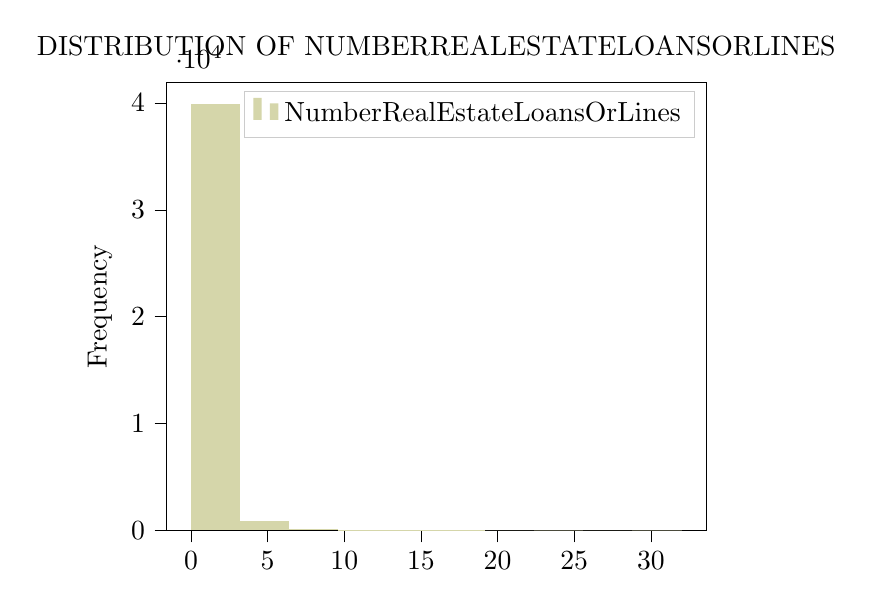
\begin{tikzpicture}

\definecolor{color0}{rgb}{0.835294117647059,0.83921568627451,0.666666666666667}

\begin{axis}[
legend cell align={left},
legend style={draw=white!80.0!black},
tick align=outside,
tick pos=left,
title={\printsubsection{\MakeUppercase{Distribution of NumberRealEstateLoansOrLines}}},
x grid style={white!69.01960784313725!black},
xmin=-1.6, xmax=33.6,
xtick style={color=black},
y grid style={white!69.01960784313725!black},
ylabel={Frequency},
ymin=0, ymax=41941.2,
ytick style={color=black}
]
\draw[fill=color0,draw opacity=0] (axis cs:0,0) rectangle (axis cs:3.2,39944);
\addlegendimage{ybar,ybar legend,fill=color0,draw opacity=0};
\addlegendentry{NumberRealEstateLoansOrLines}

\draw[fill=color0,draw opacity=0] (axis cs:3.2,0) rectangle (axis cs:6.4,918);
\draw[fill=color0,draw opacity=0] (axis cs:6.4,0) rectangle (axis cs:9.6,107);
\draw[fill=color0,draw opacity=0] (axis cs:9.6,0) rectangle (axis cs:12.8,29);
\draw[fill=color0,draw opacity=0] (axis cs:12.8,0) rectangle (axis cs:16,12);
\draw[fill=color0,draw opacity=0] (axis cs:16,0) rectangle (axis cs:19.2,4);
\draw[fill=color0,draw opacity=0] (axis cs:19.2,0) rectangle (axis cs:22.4,0);
\draw[fill=color0,draw opacity=0] (axis cs:22.4,0) rectangle (axis cs:25.6,1);
\draw[fill=color0,draw opacity=0] (axis cs:25.6,0) rectangle (axis cs:28.8,0);
\draw[fill=color0,draw opacity=0] (axis cs:28.8,0) rectangle (axis cs:32,1);
\end{axis}

\end{tikzpicture}